\let\negmedspace\undefined
\let\negthickspace\undefined
\documentclass[journal]{IEEEtran}
\usepackage[a5paper, margin=10mm, onecolumn]{geometry}
%\usepackage{lmodern} % Ensure lmodern is loaded for pdflatex
\usepackage{tfrupee} % Include tfrupee package

\setlength{\headheight}{1cm} % Set the height of the header box
\setlength{\headsep}{0mm}     % Set the distance between the header box and the top of the text

\usepackage{gvv-book}
\usepackage{gvv}
\usepackage{cite}
\usepackage{amsmath,amssymb,amsfonts,amsthm}
\usepackage{algorithmic}
\usepackage{graphicx}
\usepackage{textcomp}
\usepackage{xcolor}
\usepackage{txfonts}
\usepackage{listings}
\usepackage{enumitem}
\usepackage{mathtools}
\usepackage{gensymb}
\usepackage{comment}
\usepackage[breaklinks=true]{hyperref}
\usepackage{tkz-euclide} 
\usepackage{listings}
% \usepackage{gvv}                                        
\def\inputGnumericTable{}                                 
\usepackage[latin1]{inputenc}                                
\usepackage{color}                                            
\usepackage{array}                                            
\usepackage{longtable}                                       
\usepackage{calc}                                             
\usepackage{multirow}                                         
\usepackage{hhline}                                           
\usepackage{ifthen}                                           
\usepackage{lscape}
\usepackage{tikz}
\usepackage{textcomp}
\usetikzlibrary{circuits.ee.IEC, positioning}
\begin{document}

\bibliographystyle{IEEEtran}
\vspace{3cm}

\title{9.2.1}
\author{Manognya Kundarapu - EE24BTECH11037
}
% \maketitle
% \newpage
% \bigskip
{\let\newpage\relax\maketitle}

\renewcommand{\thefigure}{\theenumi}
\renewcommand{\thetable}{\theenumi}
\setlength{\intextsep}{10pt} % Space between text and floats


\numberwithin{equation}{enumi}
\numberwithin{figure}{enumi}
\renewcommand{\thetable}{\theenumi}
\textbf{Question:} Check if the differential equation $\frac{d^2y}{dx^2}-\frac{dy}{dx}=0$ has a solution $y=e^x+1$ for $y(0)=2$ and $y^\prime\brak{0}=1$.

\begin{enumerate}
    \item \textbf{Theoretical Solution:}\\ 
    \begin{align}
        \text{Taking } \frac{dy}{dx}=t;\\
        \frac{dt}{dx}-t=0\\
        \int\frac{1}{t}dt=\int dx\\
        ln\brak{t}=x+k\\
        t=Ce^x \text{ but } y^\prime(0)=1 \implies \frac{dy}{dx}=e^x\\
        \int dy=\int e^x dx\\
        \implies y = e^x+k\\
        \text{but } y(0)=2 \implies k=1\\
        \therefore y =e^x+1 \text{ is the solution under given conditions}.
    \end{align}
    \item \textbf{Using Trapezoidal Rule: }\\ 
    \begin{align}
        \text{For }\frac{dy}{dx}=f\brak{x,y}\\
         \int_{y_n}^{y_{n+1}}dy=\int_{x_n}^{x_{n+1}}f\brak{x,y}dx\\
         y_{n+1}-y_n\approx\frac{h}{2}\brak{f\brak{x_n,y_n}+f\brak{x_{n+1},y_{n+1}}}\\
         \implies y_{n+1}=y_n+\frac{h}{2}\brak{f\brak{x_n,y_n}+f\brak{x_{n+1},y_{n+1}}}\\
         \text{where } h=x_{n+1}-x_n
    \end{align}
    To solve the differential equation $y^{\prime \prime}-y^\prime=0$ numerically using the trapezoidal rule, we first need to rewrite it as a system of first-order differential equations, let $y_1=y \text{ and }y_2=y^\prime$
    \begin{align}
       y_1^\prime=y_2\\y_2^\prime=y_2
    \end{align}
    Using the trapezoidal rule, we get the difference equations;
    \begin{align}
        y_{1, n+1} = y_{1, n} + \frac{h}{2} \left( y_{2, n} + y_{2, n+1} \right)\\
        y_{2, n+1} = y_{2, n} + \frac{h}{2} \left( y_{2, n} + y_{2, n+1} \right)
    \end{align}
    Now the following steps were used:
    \begin{enumerate}
        \item Initialized $x_0=0$, $y(0)=2$ and $y^\prime(0)=1$.
        \item h was taken to be $0.001$, a small value and number of iterations was taken to be $1000$ to ensure accuracy.
        \item Now the subsequent points of the curve were generated through iterations by using the difference equations 2.8 and 2.9 .
    \end{enumerate}
    The below graph shows the comparison between the curve that is obtained theoretically and the simulation curv(numerically generated points through iterations).
\end{enumerate}
\begin{figure}[htbp]
  \centering
  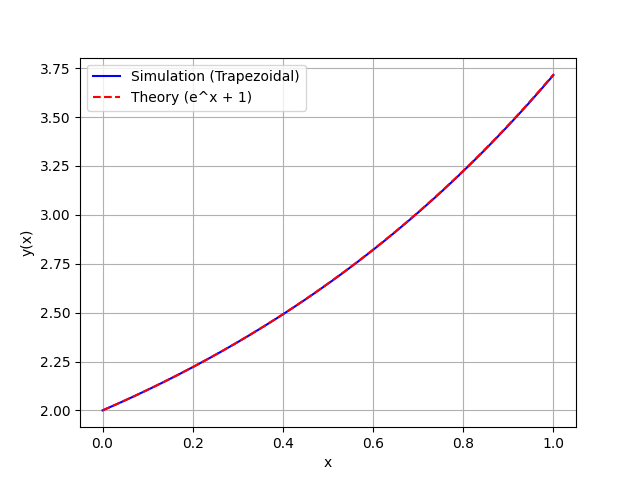
\includegraphics[width=\columnwidth]{figs/curve.png}
\end{figure}

\end{document}
  e
